% Licensed to the Apache Software Foundation (ASF) under one or more
% contributor license agreements. See the NOTICE file distributed with
% this work for additional information regarding copyright ownership.
% The ASF licenses this file to You under the Apache License, Version 2.0
% (the ``License''); you may not use this file except in compliance with
% the License. You may obtain a copy of the License at
%
% http://www.apache.org/licenses/LICENSE-2.0
%
% Unless required by applicable law or agreed to in writing, software
% distributed under the License is distributed on an ``AS IS'' BASIS,
% WITHOUT WARRANTIES OR CONDITIONS OF ANY KIND, either express or implied.
% See the License for the specific language governing permissions and
% limitations under the License.

\begin{changemargin}{1.5in}{0in}

\section{Overview}

The MetaCarta GTS appliance indexes documents and allows users to
search these documents based on both keywords and geographic
references. The MetaCarta Share Connector allows system administrators
to configure connections to network shares and define jobs to maintain
synchronization between the network shares and the GTS
index. Currently, the Share Connector supports connections to Windows Shares
and Samba shares. Limited support is available for NetApp shares.

This document specifies the means for connecting to these shares,
indexing files from these shares, and maintaining connections to
these shares.

\subsection{Assumptions}

This document assumes you have a basic level of familiarity with GTS
appliance administration. This document also assumes that you have a
basic understanding of the shared document repositories to which you
are trying to connect. If you need more information about the
MetaCarta GTS appliance, please read the \documentref{MetaCarta GTS
Administrator's Guide} stored on the appliance at
\dirpath{/usr/share/doc/metacarta/AdminGuide.pdf}. For more
information about network shares, please see your network share
documentation or network share administrator.

Throughout this document, we assume that your appliance is named \\
\url{metacarta.example.com}. 

\section{Installation}

The Share Connector is included with the Connector Addon
available from Metacarta. % Licensed to the Apache Software Foundation (ASF) under one or more
% contributor license agreements. See the NOTICE file distributed with
% this work for additional information regarding copyright ownership.
% The ASF licenses this file to You under the Apache License, Version 2.0
% (the ``License''); you may not use this file except in compliance with
% the License. You may obtain a copy of the License at
%
% http://www.apache.org/licenses/LICENSE-2.0
%
% Unless required by applicable law or agreed to in writing, software
% distributed under the License is distributed on an ``AS IS'' BASIS,
% WITHOUT WARRANTIES OR CONDITIONS OF ANY KIND, either express or implied.
% See the License for the specific language governing permissions and
% limitations under the License.

If you have not already installed the Connector Addon, you should use
the Connector Addon DVD to install it using the following steps:

\begin{enumerate}

\item Insert the DVD in your appliance.

\item Install the Connector Addon:

\begin{console}

metacarta:\~{}\$ sudo upgrade\_control install --from-dvd 

\end{console}

This will restart your appliance and eject the Connector Addon DVD.

\item Upgrade your license file, if necessary. For instructions,
see the \documentref{MetaCarta Appliance Administrator's Guide} or 
contact Customer Support (see page \pageref{SupportContact}).

\end{enumerate}

The Connector Addon cannot be uninstalled.

\subsection{Remote Updates}

In some cases, it may be very difficult to get physical access to an
appliance in order to install new software. To make the installation
process easier, MetaCarta provides a mechanism for remote
installations.  MetaCarta will provide you with ISO images of the
software you need upon request.  In brief, you can install the 
Connector Addon from ISO with the following command:

\begin{console}

metacarta:\~{}\$ sudo upgrade\_control install /path/to/iso.iso

\end{console}

For more information on the use of ISO
images for remote installations, see the \documentref{MetaCarta GTS
Administrator's Guide} stored on the appliance at
\dirpath{/usr/share/doc/metacarta/AdminGuide.pdf}.


\section{Configuration}

\subsection{Access to the Connector}

The administrator to the Share Connector % Licensed to the Apache Software Foundation (ASF) under one or more
% contributor license agreements. See the NOTICE file distributed with
% this work for additional information regarding copyright ownership.
% The ASF licenses this file to You under the Apache License, Version 2.0
% (the ``License''); you may not use this file except in compliance with
% the License. You may obtain a copy of the License at
%
% http://www.apache.org/licenses/LICENSE-2.0
%
% Unless required by applicable law or agreed to in writing, software
% distributed under the License is distributed on an ``AS IS'' BASIS,
% WITHOUT WARRANTIES OR CONDITIONS OF ANY KIND, either express or implied.
% See the License for the specific language governing permissions and
% limitations under the License.

must have
access to the web interface at
\url{http://metacarta.example.com/crawler/}. In the default appliance
security setup, you must have a Basic Authentication account
configured for access to the Connector web interface at
\url{http://metacarta.example.com/crawler/}.  If you are not an appliance
administrator, please ask the appliance administrator to give you such
an account.

An appliance administrator can create an account with access to the
ingestion interface (in this case, username {\tt fred} and password
{\tt ginger}) by running the following command on the appliance:

\begin{console}
metacarta:\~{}\$ basic\_auth\_control add ingest\_users fred:ginger 
\end{console}

Depending on how you have configured authentication using the
\command{auth\_control} tool, you may need to make changes other than
adding yourself to the ingest\_users group. For more information on
security configuration and \command{auth\_control}, see the Security
Administration section of the \documentref{MetaCarta Appliance
Administrator's Guide}.


\subsection{Initial Network Setup}

% Licensed to the Apache Software Foundation (ASF) under one or more
% contributor license agreements. See the NOTICE file distributed with
% this work for additional information regarding copyright ownership.
% The ASF licenses this file to You under the Apache License, Version 2.0
% (the ``License''); you may not use this file except in compliance with
% the License. You may obtain a copy of the License at
%
% http://www.apache.org/licenses/LICENSE-2.0
%
% Unless required by applicable law or agreed to in writing, software
% distributed under the License is distributed on an ``AS IS'' BASIS,
% WITHOUT WARRANTIES OR CONDITIONS OF ANY KIND, either express or implied.
% See the License for the specific language governing permissions and
% limitations under the License.

If you want to enforce Active Directory security on documents crawled
from \ifDocumentumGuide Documentum,\fi \ifLivelinkGuide Livelink,\fi
\ifShareGuide your network share,\fi \ifCombinedConnectorGuide your
repositories,\fi you must configure your appliance for Active
Directory support. Ask your administrator whether or not your
appliance is configured to use Active Directory.

For more information on this step, please see the \documentref{MetaCarta
GTS Administrator's Guide}, located on the appliance at
\dirpath{/usr/share/doc/metacarta}\linebreak\dirpath{
/AdminGuide.pdf}.


\section{Collecting Documents From Repositories} % Retitle this, yo.

The Connector Framework manages retrieving documents from different
repositories through \emph{jobs}. Jobs can be scheduled to run
regularly; each job connects to a single repository using a particular
set of credentials. Each job is tied to a \emph{repository
connection}. Repository connections contain information allowing the
connector framework to connect to a given repository, in this case a
given network share. A repository connection may be tied to an
\emph{authority connection}, which manages document security. While
using the Share Connector to connect to a network share, no authority
connection is needed; you can simply create a repository connection.



\subsection{Creating Repository Connections}

In order to create jobs to ingest documents, you need to create a
repository connection. To do so, click ``List Repository
Connections'' on the sidebar menu. Then, when presented with the list
of repository connections, click ``Add a new connection.'' You will
see the following two tabs:

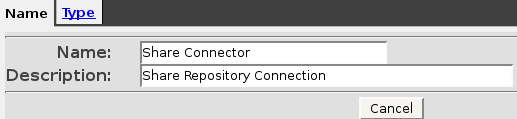
\includegraphics[width=300pt]{Share-edit-repository-tab1}

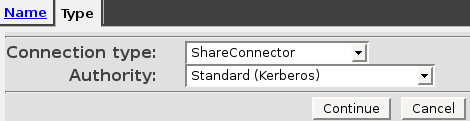
\includegraphics[width=300pt]{Share-edit-repository-tab2}

% Licensed to the Apache Software Foundation (ASF) under one or more
% contributor license agreements. See the NOTICE file distributed with
% this work for additional information regarding copyright ownership.
% The ASF licenses this file to You under the Apache License, Version 2.0
% (the ``License''); you may not use this file except in compliance with
% the License. You may obtain a copy of the License at
%
% http://www.apache.org/licenses/LICENSE-2.0
%
% Unless required by applicable law or agreed to in writing, software
% distributed under the License is distributed on an ``AS IS'' BASIS,
% WITHOUT WARRANTIES OR CONDITIONS OF ANY KIND, either express or implied.
% See the License for the specific language governing permissions and
% limitations under the License.

\begin{picture}(1,1)
  \put(-100,15){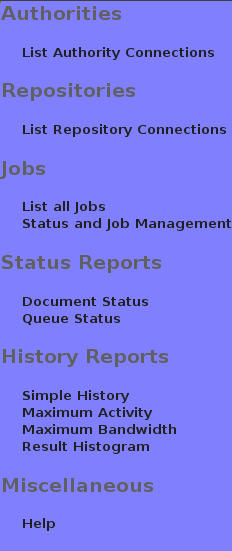
\includegraphics[width=80pt]{crawler-sidebar}}
\end{picture}


Now you must provide a name, description, and connector type for your
new repository connection. The name should be unique, as you will use
it to select this connection later when defining jobs. The description
should explain the repository connection to you or another
administrator.  The connector type is the type of repository from
which you will get documents, in this case a ShareConnector. The
authority type is the type of authority from which you will get
authorization information. The Share Connector does not use an
administrator-created authority; you should simply select ``Standard
(Kerberos)'' here.

Once you have filled in those tabs, click ``Continue'' to be taken to
the repository-specific options.

% Licensed to the Apache Software Foundation (ASF) under one or more
% contributor license agreements. See the NOTICE file distributed with
% this work for additional information regarding copyright ownership.
% The ASF licenses this file to You under the Apache License, Version 2.0
% (the ``License''); you may not use this file except in compliance with
% the License. You may obtain a copy of the License at
%
% http://www.apache.org/licenses/LICENSE-2.0
%
% Unless required by applicable law or agreed to in writing, software
% distributed under the License is distributed on an ``AS IS'' BASIS,
% WITHOUT WARRANTIES OR CONDITIONS OF ANY KIND, either express or implied.
% See the License for the specific language governing permissions and
% limitations under the License.

\subsubsection{Configuring a Share Connection}

You must fill in the following tabs if you are configuring a Share
connection:

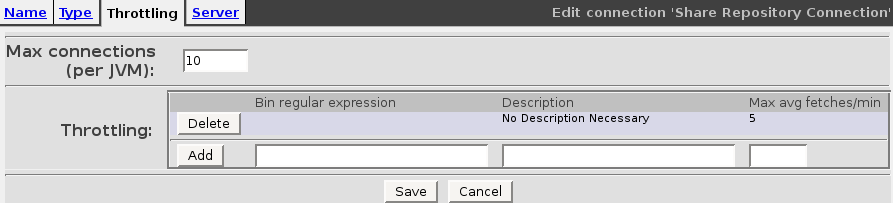
\includegraphics[width=300pt]{Share-edit-repository-tab3}

\begin{itemize}

\item \textbf{Max connections (per JVM):} Here you can set the maximum
number of connections to your repository.  \ifCombinedConnectorGuide
The maximum number of connections per JVM is important for three
reasons; licensing, appliance resources, and the possiblity of
overwhelming the ingestion interface. For a more complete explanation,
see the Max Connections item on page \pageref{maxrepocon}.\fi

\ifShareGuide
The maximum number of connections per JVM is important for three reasons.
First, the number of connections may impact the licensing on your document
server, depending on the repository.

Second, the number of connections may impact the resources
available on the appliance. If the connector framework is slowing down
your appliance, lowering this number should help.

Third, only ten document streams can be processed by the appliance
at one time.  If you are also using other repository connectors or
the \command{ingest} command on the appliance, you should reduce this
number to prevent contention for the Ingestion interface. The Share
Connector will never overwhelm the interface on its own, but when other
applications are also using the ingestion interface, it may be best to
set the number of repository connections to five or even fewer.
\fi

\item \textbf{Throttling:} Here you can set a maximum document fetch
rate for the repository connection.


The maximum fetch rate allows you to set three things: Expression,
description, and fetches per minute. Expression allows you to provide
a regular expression to match against document bins.  Each document
ingested through a connector is associated with one or more document
bins. These bins represent the servers that the connector interacts
with to obtain the document.  Typically, a document will be associated
with only one document bin, representing the repository server hosting
the document. For some repository connections, documents ingested
through the connector can be hosted by different servers. In the Share
Connector, documents only come from one server, which you will set on
the following tab. Simply leave the expression blank; this will match
any server you enter on the following tab.  All you need to set is the
number of document fetches per minute.  Description is an optional
field that allows you to provide a short text description of the
throttle.  Once you have set the fetch rate and optional description,
click Add.




\end{itemize}

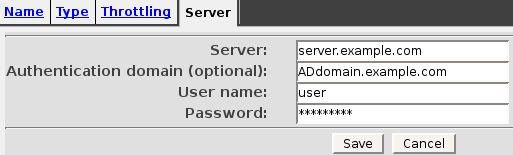
\includegraphics[width=300pt]{Share-edit-repository-tab4}

\begin{itemize}

\item \textbf{Server:} The fully qualified sever name of network share
with which you wish to connect.

\item \textbf{Authentication domain (optional):} The Active Directory
domain that your network share is a part of. This is an optional
argument. 

\item \textbf{User name:} The user name that the GTS appliance will
use to connect to the network share for this repository connection.
Typically, your network share administrator will create this account
specifically for use by the appliance. The account used by the GTS
appliance must have sufficient authority to retrieve files and their
corresponding ACLs.

\item \textbf{Password:} The password corresponding to the
user name given to the GTS.

The Active Directory domain should only be included once between the
``Authentication domain'' and ``User name'' fields, but may not be
necessary for either. The exact phrasing required by the crawler
depends on the configuration of your network share. This is a common
cause of a failed repository connection. In order to correctly
configure your repository connection you may need to try all 3
possible pairings: \command{ADdomain.example.com} with \command{user}, a
blank domain with \command{user@ADdomain.example.com}, and a blank
domain with \command{user}.

\end{itemize}

\note{The Share Connector gets its domain authentication information by
querying the relevant AD domain for a list of domain controllers and
then trying the first domain controller on that list. If your domain
controllers are inaccessible, the Share Connector will not be able to
function.} 

% This should go in a Troubleshooting section when we have one,
% but rc4 is not the time.

After entering this information, you will be taken to the repository 
connection status page for this repository:

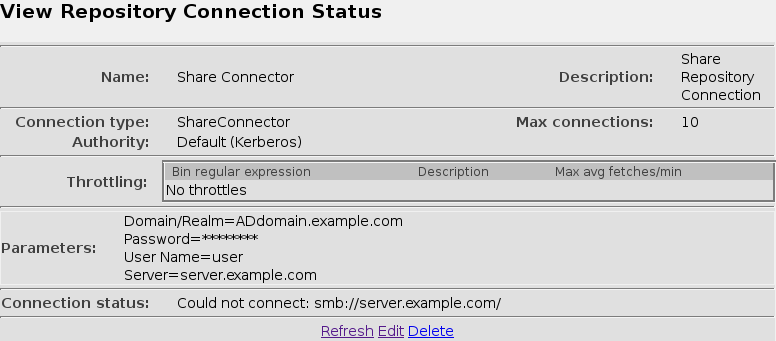
\includegraphics[width=300pt]{Share-view-repo-conn-status}

In this example (which does not contain accurate information for any
Share Connector), the Connection Status is ``Connection failed.''  If
you see this message, you most likely have incorrectly entered one of
the fields, and should click ``Edit'' to fix the data. If you have
entered everything as you intended, please inform your network share
administrator; you may not have been given the correct information.


\subsection{Creating and Running Jobs}

To run a job, click ``Status and Job Management'' on the sidebar menu.
You can run or edit existing jobs from this menu.

To create a new job, click ``List All Jobs'' on the sidebar menu. Then, when
presented with the list of current jobs, click ``Add a new job.'' You
will be presented with two tabs, in which you must fill in the following
information:

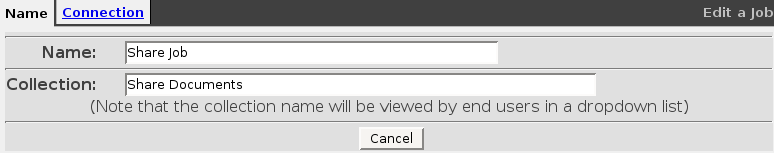
\includegraphics[width=300pt]{Share-edit-job-tab1}

\begin{itemize}

\item \textbf{Name:} The name of the job. You will use this to identify
the job later.

\item \textbf{Collection:} The collection name metadata for all
documents in this job. End users can use this name to select the set
of documents in this job. For more information on collection name
metadata, please see the \documentref{MetaCarta GTS Administrator's
Guide}.

\end{itemize}

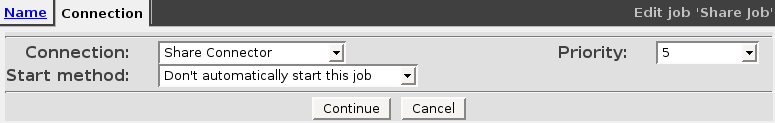
\includegraphics[width=300pt]{Share-edit-job-tab2}

\begin{itemize}

\item \textbf{Connection:} The name of the repository connection you
wish to use for this job. You select this from the list of repository
connections you have already made. You may have more than one job use
the same repository connection, but if you have two jobs crawl the same
documents, the documents will have the metadata and collection name
associated with whatever job crawled the document most recently. This
will cause unpredictable results when searching those collections,
searching for those documents, or trying to delete those collections.
We recommend never crawling the same document in two different jobs.

\item \textbf{Start method:} Whether you want to start this job the next
time jobs are scheduled to run (``Start when schedule window starts''),
immediately after you finish defining it (``Start even inside a schedule
window''), or not at all (``Don't automatically start this job'').

\item \textbf{Priority:} From 1 (highest) to 10 (lowest), the priority
this crawl should have if it must compete for resources with other
crawls on the appliance. You should not need to change this unless you
are running more than one crawl at the same time; if you are, assign a
higher priority to the crawls whose documents you want to be processed
preferentially before documents from other jobs.

\end{itemize}


After filling in those options, click ``Continue'' and you will be
presented with repository-specific options.

% Licensed to the Apache Software Foundation (ASF) under one or more
% contributor license agreements. See the NOTICE file distributed with
% this work for additional information regarding copyright ownership.
% The ASF licenses this file to You under the Apache License, Version 2.0
% (the ``License''); you may not use this file except in compliance with
% the License. You may obtain a copy of the License at
%
% http://www.apache.org/licenses/LICENSE-2.0
%
% Unless required by applicable law or agreed to in writing, software
% distributed under the License is distributed on an ``AS IS'' BASIS,
% WITHOUT WARRANTIES OR CONDITIONS OF ANY KIND, either express or implied.
% See the License for the specific language governing permissions and
% limitations under the License.


\subsubsection{Share Job Options}

You must complete the following tabs to configure a Share Job:

\bigimage{Share-edit-job-tab3}


\ifShareGuide
% Licensed to the Apache Software Foundation (ASF) under one or more
% contributor license agreements. See the NOTICE file distributed with
% this work for additional information regarding copyright ownership.
% The ASF licenses this file to You under the Apache License, Version 2.0
% (the ``License''); you may not use this file except in compliance with
% the License. You may obtain a copy of the License at
%
% http://www.apache.org/licenses/LICENSE-2.0
%
% Unless required by applicable law or agreed to in writing, software
% distributed under the License is distributed on an ``AS IS'' BASIS,
% WITHOUT WARRANTIES OR CONDITIONS OF ANY KIND, either express or implied.
% See the License for the specific language governing permissions and
% limitations under the License.

\begin{itemize}
\label{scheduling}

\item \textbf{Schedule type:} Whether you want to scan every document
once or dynamically recrawl content in your repository. 

When scanning every document once, the crawler marks all documents that
have been previously crawled in this job as potentially to be deleted,
adds all seed documents to its queue and marks them as pending, processes
pending documents, marking them completed as they are ingested, and then
deleted all of the documents that were not recrawled. A document might
not be recrawled because it no longer exists, or the job specification
might have been changed to no longer include the document.

When dynamically recrawling documents, the crawler does not start by
marking all documents as potentially deletable; instead, it begins with
all of the seed documents, and continues adding to its list, periodically
re-adding the initial seed documents. If a document is removed from the
source, it will expire in the expiration interval (see below).

\item \textbf{Expiration Interval (if continuous):} The length of the
interval (in minutes) that the appliance will retain a document
crawled by this job after the document no longer appears in the
repository. After this interval, the missing document will be removed
from the appliance's index and archive. Leave the expiration interval
blank to keep missing documents indexed in GTS.

\item \textbf{Recrawl interval:} If you are dynamically recrawling
documents, how long, in minutes, the crawler should wait before
crawling documents a second time.

\item \textbf{Reseed interval:} If you are dynamically recrawling
documents, how long, in minutes, the crawler should wait before
looking for new documents to crawl. \ifMeridioGuide This connector
identifies all documents for ingestion through seeding; if the reseed
interval is infinite, the job will not ingest documents placed in the
repository during run time. (The job automatically reseeds whenever it
is started.) The default interval of 60 minutes is an appropriate
reseed rate. \fi \ifFilenetGuide This connector identifies documents
for ingestion during seeding. If you change the document inclusion
criteria, reseeding is required to identify new documents. Similarly,
documents placed in the repository while the job is running will not
be identified until the crawl is reseeded.  (The job automatically
reseeds whenever it is started.) The default interval of 60 minutes is
an appropriate reseed rate. \fi

\item \textbf{Scheduled time:} Allows you to define a time you wish
the job to run using a series of selection boxes. The first box refers
to the day of the week you wish the job to run, with an option to have
the job run any day of the week. The second box allows you to select
the start hour, with an option to start the job at any hour. The third
box allows you to specify which minute after the hour that you wish
the job to start. The fourth box allows you to specify what months of
the year you wish the job to run, with an option for the job to run
any month. The last box allows you to specify the day of the month you
wish the job to start, including any day of month.


You can scroll through each of the five boxes in this setting using
the arrow keys on your keyboard or by using the scroll bar on the
right side of the box.  If you want to select more than one value,
hold down control as you scroll and click the values that you want to
select. This allows you to define multiple windows with the same
length, for example by selecting Monday, Wednesday, and Friday at the
same time.

\item \textbf{Maximum run time:} The longest you will allow the job to
run, in minutes. For example, if you want to start a job at 2 AM but
force it to stop at 8 AM so that users have access to the repository,
you should set this value to 360 minutes. If the job is not complete by the
end time, documents that have already been found will be indexed, and
the rest of the crawl will continue at the beginning of the next
schedule interval. 

When you have defined the scheduled time and assigned a maximum run
time, click on the ``Add Scheduled Time'' button. A new schedule box
will appear below the scheduled time, allowing you to create
additional scheduled run times.

Here is a sample schedule for a job that will run every
Monday from 2 am to 6 am:

\begin{changemargin}{-.3in}{0in} 
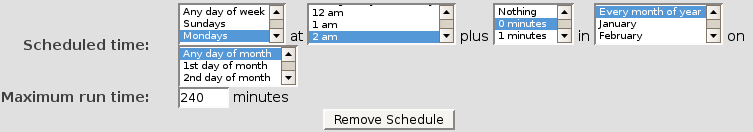
\includegraphics[width=300pt]{sample-schedule}
\end{changemargin}

If you do not have at least one scheduled time, the job will
only run when run manually (see page \pageref{ManageJobs}), and will
not automatically update the index on the appliance based on changes
to the repository.

You can remove a scheduled time by clicking the ``Remove Schedule''
button.

\end{itemize}

\fi

\ifCombinedConnectorGuide
This tab presents scheduling options. Here you can generate one or
more scheduled run times for the job. For a complete description of
the scheduling options, see the description starting on page
\pageref{scheduling}.
\fi


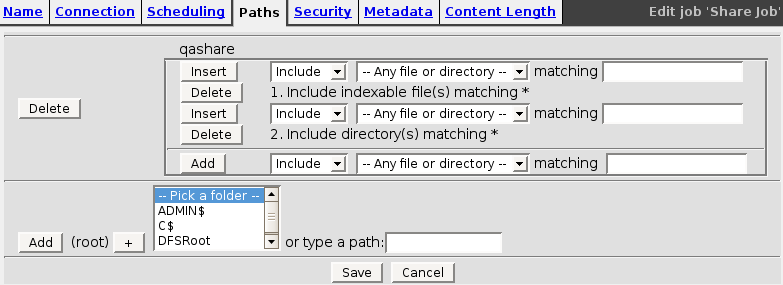
\includegraphics[width=300pt]{Share-edit-job-tab4}

\begin{itemize}

\item \textbf{Paths:} Here you can specify directory and file paths in
your network share from which you want your crawl to start. You can
specify one or more paths. If you do not specify any paths, the job
will not crawl any directories or documents. To generate each set of
paths, you must first build a directory path. You can build a
directory path by selecting individual directories. To start, you can
either select the base directory from the selection box or, if it does
not appear in the selection box, type its name in the empty text box,
then click the ``+'' button. A new selection box will appear with the
directories contained by that parent directory, along with a new text
box. Select or fill in a directory at that level and click the ``+''
button. Continue building your directory path in this fashion. When
it's complete, click ``Add''.

The directory path will appear along with a crawl customization
box. Using this customization box, you can use Windows file matching
expressions (or ``wildcard expressions'') to further specify directory and
file paths to crawl. Each path customization includes three parts. The
first selection is used to include or exclude items matched by a
wildcard expression. The second selection allows you to specify what
types of files and/or directories should be included with this
customization. The last part is a text box in which you can enter a
wildcard expression used to match files and/or directories. Complete
all three fields and click ``Add'' to insert the wildcard expression
instruction at the end of the list of instructions.

The list of wildcard expression instructions is evaluated from top to
bottom. Customization boxes appear in between list items, allowing the
insertion of instructions into the list. A wildcard expression
instruction can be deleted from the list by clicking the ``Delete''
button that appears next to it. By default, the list of instructions
includes two statements, \command{1.~Include file(s) matching *} and
\command{2.~Include directory(s) matching *}. Together these
instructions tell the job to crawl all contents contained by the
parent directory path.

Wildcard expressions use wildcard characters to match file and
directory names. The character \texttt{*} is used to match any zero or
more characters, while the character \texttt{?} matches any single
character. The brackets characters \texttt{[]} match any single
selection of characters that appears within the brackets. Simply
entering \texttt{*} as an expression matches everything. Some other
possiblities:

\begin{itemize}

\item \texttt{file??.txt}: A sequence of text files with a two digit
identifier.

\item \texttt{file*.txt}: A sequence of text files with a variable
length identifier.

\item \texttt{*.txt}: Any text file.

\item \texttt{*Data}: Any directory whose name ends with the word
``Data''.

\item \texttt{[abc]*}: Any file or directory whose name begins with
``a'', ``b'', or ``c''.

\item \texttt{*.[abc]*}: Any file whose extension begins with ``a'',
``b'', or ``c''.

\end{itemize}

You can continue to add more directory paths to your list using the
new selection box that appears below your completed directory
path. Each directory path can be customized with instructions as
described above. To remove a directory path from the list, click the
``Delete'' button next to it.

\end{itemize}

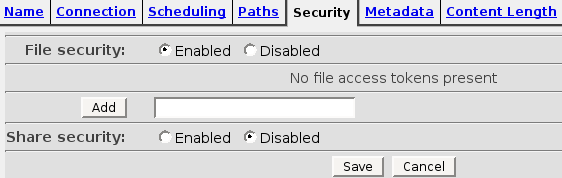
\includegraphics[width=300pt]{Share-edit-job-tab5}

\begin{itemize}

\item \textbf{File Security:}  Allows you to control whether or not file ACLs,
or access control lists, are passed to the appliance with the files.

\item \textbf{Access Tokens:} If you want to pass on your own Active
Directory ACLs instead of those of the network share you can enter
them here. You should enter one or more SIDs that you want to have
read permissions on the files crawled in this job. For more
information about AD ACLs and SIDs, please see the security sections
of the \documentref{MetaCarta Appliance Administrator's Guide}.

\note{If you have disabled security, these ACLs will not be passed to
the appliance.}

\item \textbf{Share Security:} In some cases, your network share's
security may include share security. You should enable or disable
share security to match your network share's security model.

\end{itemize}

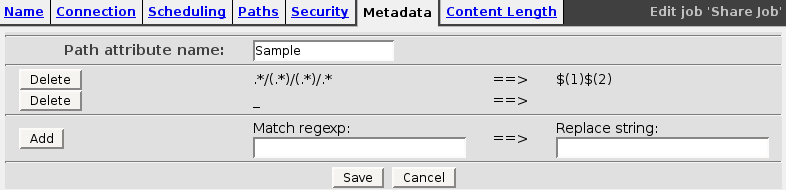
\includegraphics[width=300pt]{Share-edit-job-tab6}

\begin{itemize}

\item \textbf{Path Attribute name:} You can create a metadata field
to contain attributes from the file path. You can enter a name
for the metadata field here. It may be useful to have the metadata
field containing path attributes have the same name across jobs.
This metadata will not be geographically parsed or used to create the
index on the MetaCarta appliance; however, with MetaCarta Search APIs,
you can construct searches based specifically on this metadata. For more
information on the SOAP Search API, please see the \documentref{MetaCarta
SOAP Search API Guide}, and for more information on the JSON and KML
Search APIs, please see the \documentref{Web Services Search Guide}.

\item \textbf{Path-value mapping:}The regular expressions and
substitutions that you want to use to collect information from the
file path. You can construct one or more regular expressions. In the
example shown, there are two expressions. The first,
\verb+.*/(.*)/(.*)/.*+ to \verb+$(1) $(2)+, would change the directory
path ``Project/Folder\_1/Folder\_2/ Filename'' into ``Folder\_1
Folder\_2.'' The second, \_ to a space, would then be applied to turn
the metadata into ``Folder 1 Folder 2.'' It is important to allow more
than one transform so that you can, if necessary, extract text data
and then parse the extracted data. The end result of the last
transform will be ingested as the value of the metadata attribute
defined previously. \ifCombinedConnectorGuide If you are not familiar
with regular expressions, please see the note on page \pageref{regex}
for more information.\fi

\ifShareGuide 
\label{regex} 

\note{If you are not familiar with regular expressions, there
are a variety of tutorials available on the web, including
\url{http://gnosis.cx/publish/programming/regular_expressions.html}
and \url{http://}\linebreak \url{perldoc.perl.org/perlrequick.html}. If
you still have difficulty with these settings, please contact Customer
Support (see page \pageref{SupportContact}).} 

\fi

\end{itemize}

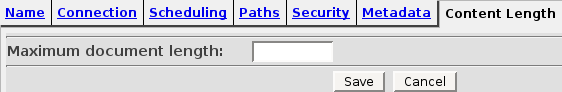
\includegraphics[width=300pt]{Share-edit-job-tab7}

\begin{itemize}

\item \textbf{Content Length:} The maximum file size, in bytes, that
you wish this job to crawl. Files larger than this size will be
skipped. The default maximum content length is unlimited.


After entering this information, you will be taken to the status page
for this job:

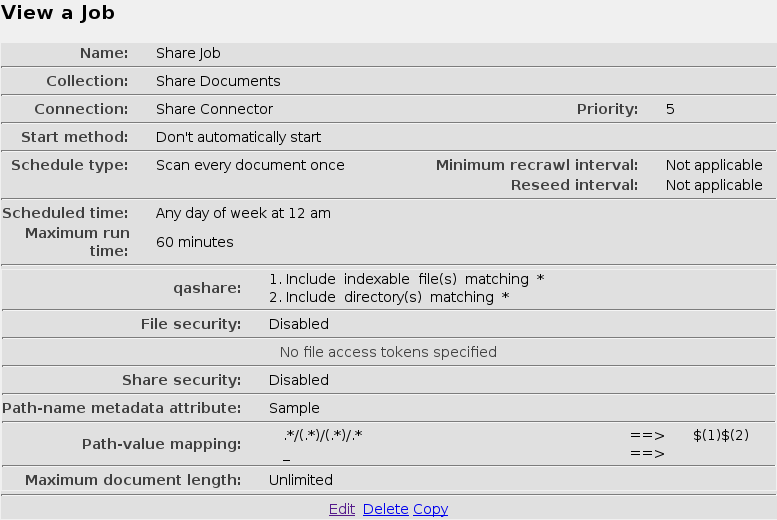
\includegraphics[width=300pt]{Share-view-job-status}


\end{itemize}



\subsection{\label{ManageJobs}Status and Job Management}

You can then look at the status of your job by clicking ``Status and 
Job Management'' on the sidebar. You will see a list of one or more jobs
much like this one:

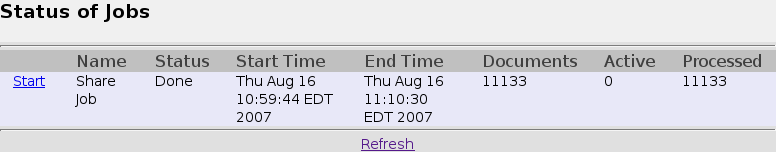
\includegraphics[width=300pt]{Share-jobs-list}

You can start any crawl you like immediately from this interface by
clicking ``Start'' next to the name of the crawl. This interface also
allows you to see how many documents have been crawled; this information
may help you structure and plan future crawls.

\note{Refresh this page by clicking the ``Refresh'' link at the bottom
of the page, not by clicking your browser's reload button.}

\section{Reports}

The Connector interface can generate four types of reports:

\begin{itemize}

\item Simple History, which lets you list an ordered set of log events
based on chosen criteria

\item Maximum Activity, which lets you see the period of time in
which a certain event happened most often

\item Maximum Bandwith, which lets you see the period of time in
which the most bandwidth was used 

\item Result Histogram, which provides log information that would be
appropriate for constructing a histogram or other diagram

\end{itemize}

Each of these reports allows you to specify a connection, one or more
activities, a start time, an end time, an entity match, and a result code
match.  Some also allow you to specify an identifier class description
and a sliding window size. This section will show sample results for
each type of report and an explanation of the fields selected.

\subsection{Simple History}

This report was generated by selecting ``Share Repository Connection,'' 
clicking Continue, selecting ``document ingest,'' and clicking Go.

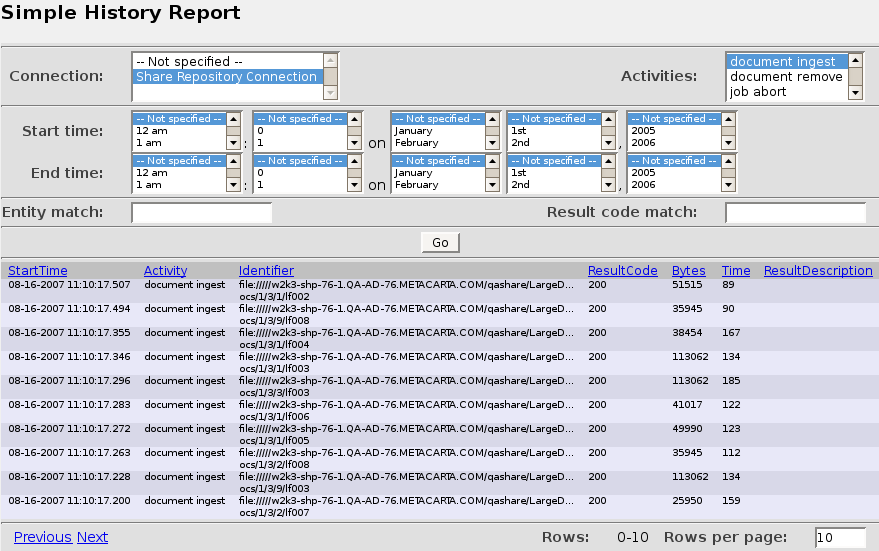
\includegraphics[width=300pt]{Share-simple-history-report}

\begin{itemize}

\item \textbf{Connection:} The repository connection from which to generate
a report.

\item \textbf{Activities}: What crawler activities you would like to see. 
Your options are document ingest, document remove, fetch document, find 
documents, job abort, job continue, job end, job start, and job wait. 

\item \textbf{Start time}: The earliest time in the crawler logs to be
considered for this query.  Choose ``Not specified'' for any field to
start at the beginning of the crawler's logs.

\item \textbf{End time:} The latest time in the crawler logs to be
considered for this query. Choose ``Not specified'' for any field 
to end at the current time.

\item \textbf{Entity match:} A regular expression to limit the
Identifier field. If the entity match field in the example above had
been \texttt{\^{}17}, only document fetches with Identifiers starting
with 17 would be shown.

\item \textbf{Result code match:} A regular expression to limit the
ResultCode field.

\end{itemize}

You can sort the history report by any of the returned fields; to do so,
click the field names.

\subsection{Maximum Activity}

This report was generated by selecting ``Share Repository Connection,''
clicking Continue, selecting ``document ingest,'' changing the Identifier
class description, and clicking Go.

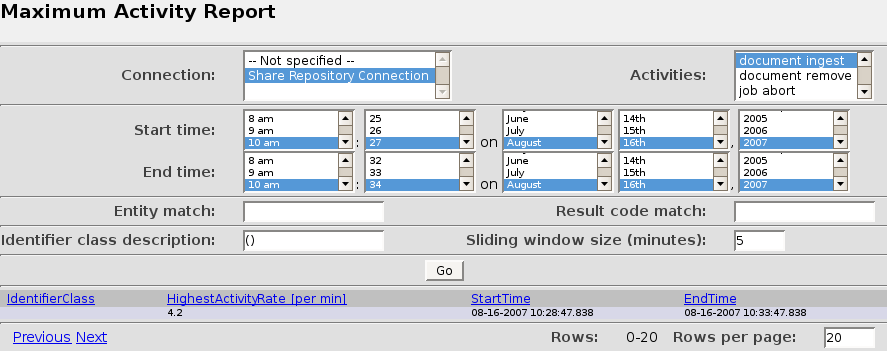
\includegraphics[width=300pt]{Share-maximum-activity-report}

This form offers two more fields than the previous form:

\begin{itemize}

\item \textbf{Identifier class description:} A regular expression
that determines how to group identifiers together. If this were set to
\texttt{(.*)}, there would be no grouping, and so there would be only one
ingestion event per document. If this were set to \texttt{(17)},
then all documents with identifiers beginning with 17 would be grouped
together. The setting in the example, \texttt{()}, groups all
documents together. Some other possibilities:

\begin{itemize}

\item \texttt{1(.)}: (up to) Ten groups of documents whose identifier starts
with 1, labeled 0-9, grouped by the second digit of their identifier.

\item \texttt{()}: One group of documents containing all documents 
regardless of identifier.

\item \texttt{17}: One group of documents whose identifier contains
the string ``17.''

\item \texttt{\^{}17}: One group of documents whose identifier \emph{starts}
with the string ``17.''

\end{itemize}

\item \textbf{Sliding window size}: The search interval in minutes.

\end{itemize}

The report returned will have only one result per group with one or more
documents in it, if there is a clear highest activity rate, or a list of
all the results tied for highest activity rate if there are more than one.

\subsection{Maximum Bandwidth}

This report was generated by selecting ``Share Repository Connection,''
clicking Continue, selecting ``document ingest,'' changing the Identifier
class description, and clicking Go.

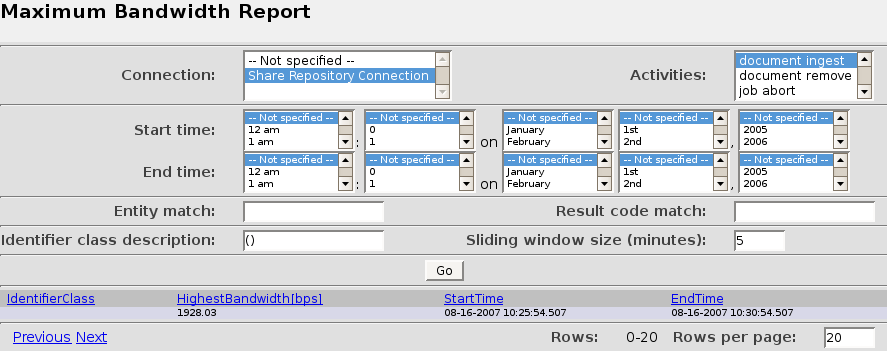
\includegraphics[width=300pt]{Share-maximum-bandwidth-report}

This form offers the same fields as the maximum activity form, and
returns similar results; instead of tracking events per time window,
it tracks the window with the highest average bandwith usage, measured
in bytes per second. Again, the identifier class description has been
changed to a regular expression that will match all identifiers (and
thus in this case documents).

\subsection{Result Histogram}

This report was generated by selecting ``Share Repository Connection,''
clicking Continue, selecting ``document ingest,'' and clicking Go.

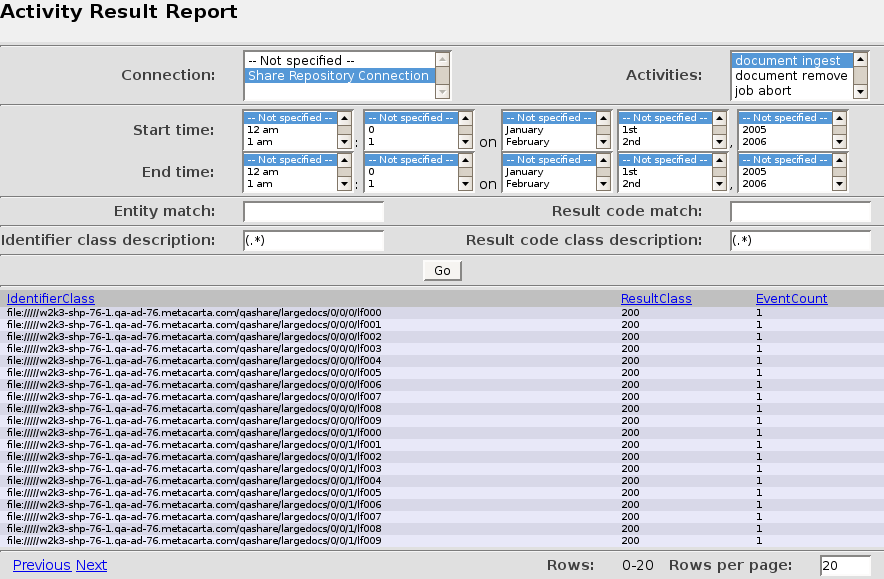
\includegraphics[width=300pt]{Share-activity-result-report}

This form adds one new field:

\begin{itemize}

\item \textbf{Result code class description:} A regular expression that
determines how to group result classes together; like Identifier class
descriptions but for result classes.

\end{itemize}

This report does not produce an actual histogram, but provides data that
could be used to generate histograms.  

% This is a little sparse, but that's basically all this is, so.

\end{changemargin}
